%Reliability
Today, reliability is being explored at different layers of abstraction; from devices to memory to algorithms.
At a circuit-level, ~\cite{chen2015fast} uses a conditional probability approach for modeling reliability in combinational circuits.
Approximate computing is being considered one of the potential pathways in reducing energy inefficienices in applications that can tolerate some amount of error.
~\cite{chippa} uses scalable effort hardware for the design of efficient hardware implementations for algorithms that demonstrate inherent error resilience.
In ~\cite{temam2015}, the authors propose an inexact neural network accelerator with significant energy savings.
In this section, we evaluate the capabilities of a bio-inspired visual object recognition algorithm - HMAX - and leverage its potential to save 
power and reduce computational resources. 

\subsection{HMAX}
The first few hundreds milliseconds of visual processing in primate
cortex mostly follows a feedforward hierarchy and in ~\cite{serre}, the authors proposed such a hierarchical visual object recognition model - HMAX - that consists of 
four layers of alternating units of \textit{simple} \textbf{S} and \textit{complex} \textbf{C} units. 
This model was further refined in ~\cite{Mutch2008} where the inputs to 
the second S layer i.e. ``S2'' are sparsified. For further insights, we point readers to ~\cite{poggio} where the claim made is 
that a hierarchical MAX-like operation is a key mechanism for object recognition in the cortex.
HMAX while being computationally expensive is highly parallel and various accelerator designs have been proposed for 
embedded real-time applications~\cite{Kestur2012, Maashri2012a}. 
All our experiments in this work are based on \textit{hmin} - a publicly available representation of HMAX~\cite{hmin}.

\subsection{Exploiting Resiliency for Power Benefits}

So far we have surveyed the landscape of vision systems that enhance the 
performance and energy efficiency of the computational fabrics. 
However, memory is an integral part of most systems today and contributes 
between 10-30\% of the overall power of embedded video systems and 
mobile phones~\cite{CarrollAaronHeiser2010}. Propeilled by the growth in big data, the demand for cloud storage is allowing for larger DRAM devices to be used today. 
However data in every DRAM cell needs to be refreshed periodically to maintain integrity. This is done by reading a row and writing it back 
from the sense amplifier. JEDEC standards~\cite{jedec-sdram-standards} define a 64 ms refresh window in which a maximum of 8192 refresh commands are issued via an auto-refresh command by the memory controller. 
The increasing memory size has made DRAM memory refresh energy a matter of growing concern and new 
power-efficient techniques such as Low Power Auto Self Refresh, Temperature Controlled Refresh, Refresh Pausing, Fine Granularity Refresh and Data Bus 
Inversion have been introduced in recent memory standards such as DDR4~\cite{jedec-sdram-standards}.

Modulating DRAM refresh based on the data characteristics has been proposed as early as 1998~\cite{islped98}.  
In ~\cite{Liu2011}, the authors looked at reducing refresh power on multimedia workloads. Recently, in ~\cite{iccd2014}, the authors showed that 
refresh power can dynamically be changed based on autonomously tagging data with logical labels.
Many recent works have looked at tackling the increasing refresh power in other 
different ways. ~\cite{Liu2012} used software techniques while in ~\cite{Stuecheli2010}, scheduling 
policies were proposed, and ~\cite{Nair2013} used a refresh pausing mechanism to
exploit idle memory cycles.
Very recent work suggests a Flexible Auto-Refresh scheme to 
skip unneeded refreshes in DRAMs~\cite{isca2015}.

In this section, we showcase a data-dependent method to reduce refresh rates. 
More specifically, we explore the resiliency of HMAX to bit errors, which can then be used to choose the refresh rate for DRAM-based memory storage.  
As shown in Fig.~\ref{tab:hmax_reliability}(a), we choose six classes from the CalTech101 dataset~\cite{Fergus2004} 
and obtain a recognition accuracy of around 78\%. Next we introduce salt and pepper noise into 128 pixels of each testing image 
as shown in Fig.~\ref{tab:hmax_reliability}(b). This noise corresponds to 1024 cell failures in a 32GB DRAM device~\cite{Liu2012}. 
We find that the accuracy drops by less than 1\%. 
Based on the cumulative cell failure probability curve provided in ~\cite{Liu2012}, this implies 
that by increasing the refresh period from 64ms to 256ms we can expect up to 1000 cell failures in a 32GB DRAM device. Under these constraints, HMAX will 
still maintain recognition rates within a 1\% error bound, thus helping in reducing the overall refresh energy.

Fig.~\ref{fig:hmax_pixel_sensitivity} illustrates the classification accuracy of HMAX as a 
function of the pixel errors introduced in each image.
We find that HMAX is resilient to up to 512 pixel errors after which there is a roll-off in accuracy. 
We also inspected the accuracy function for each of the six classes independently and found that each class had its own sensitivity curve. This observation suggests 
that having a data-dependent differential refresh scheme as proposed in ~\cite{iccd2014} would help in further reducing refresh energy.

%HMAX Expt
\begin{figure*}[!htb]
\centering
\begin{tabular}{@{}c@{} @{}c@{}}
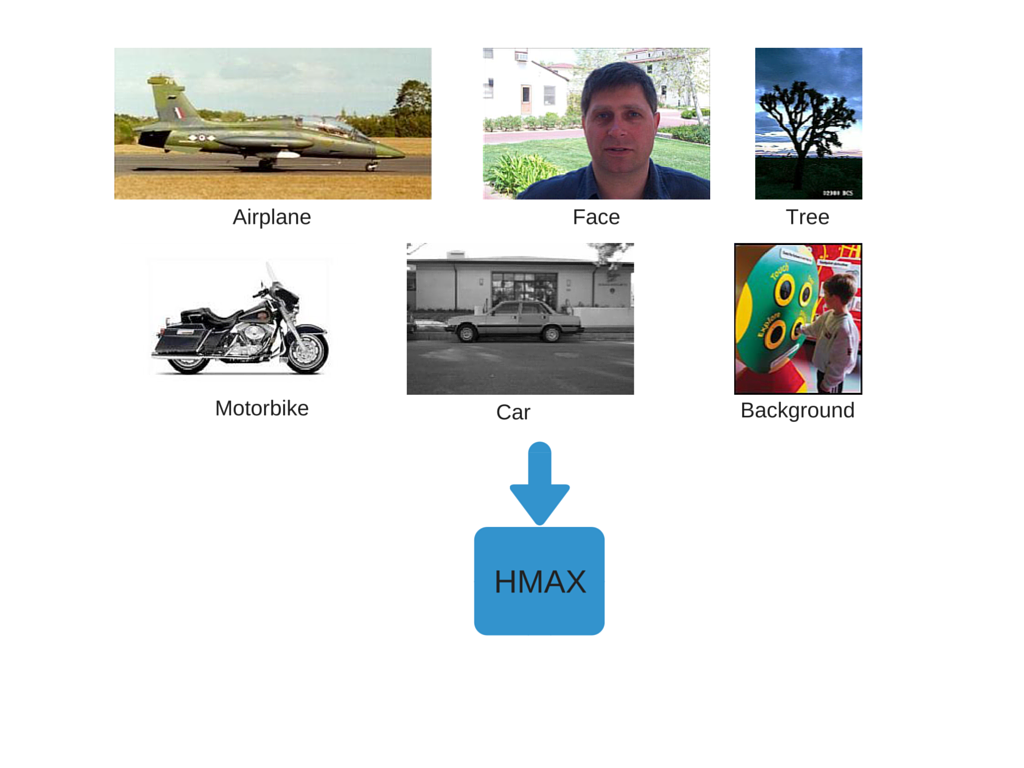
\includegraphics[width=0.45\linewidth]{./figures/hmax_reliability_a.png} & 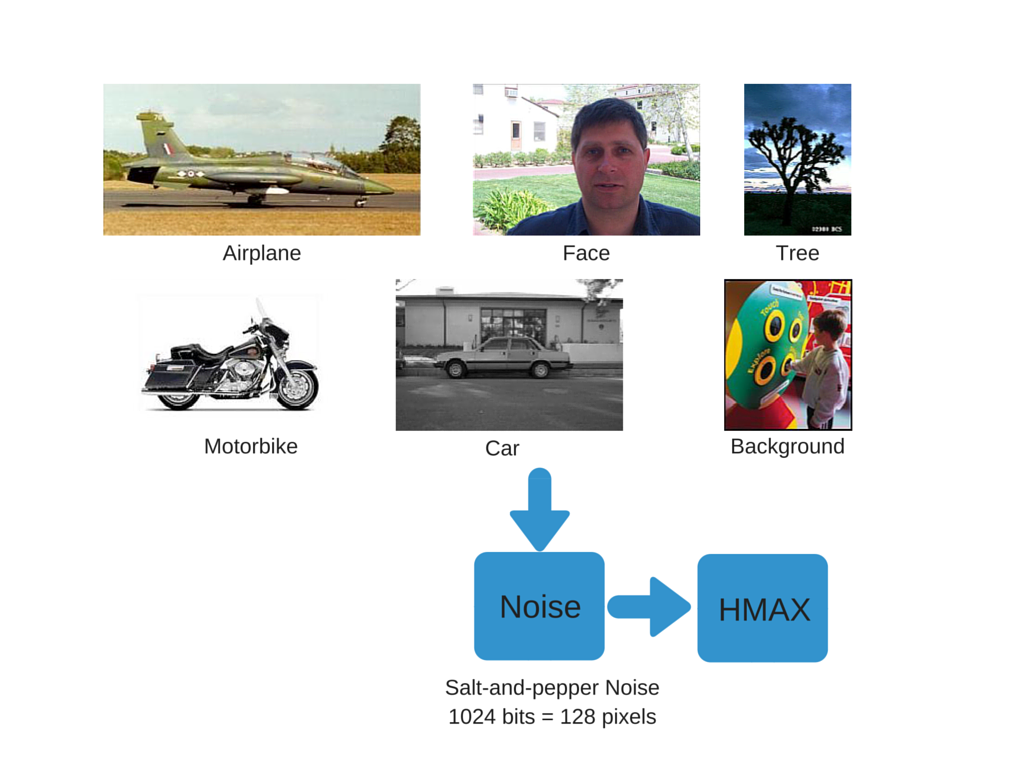
\includegraphics[width=0.45\linewidth]{./figures/hmax_reliability_b.png}\\[\abovecaptionskip]
\small (a) Baseline & \small (b) Noise
\end{tabular}
\vspace{1pt}
\caption{HMAX resilience to errors. Six classes from CalTech101 were used. We use (a) as our baseline. Since HMAX operates only on grayscale image, we convert each image to grayscale (8 bits) before processing. In (b) we introduce salt and pepper noise in 128 pixels as shown.}
\label{tab:hmax_reliability}
\end{figure*}

%HMAX Resilience
\begin{figure}[htb!]
\vspace{0pt}
\centering
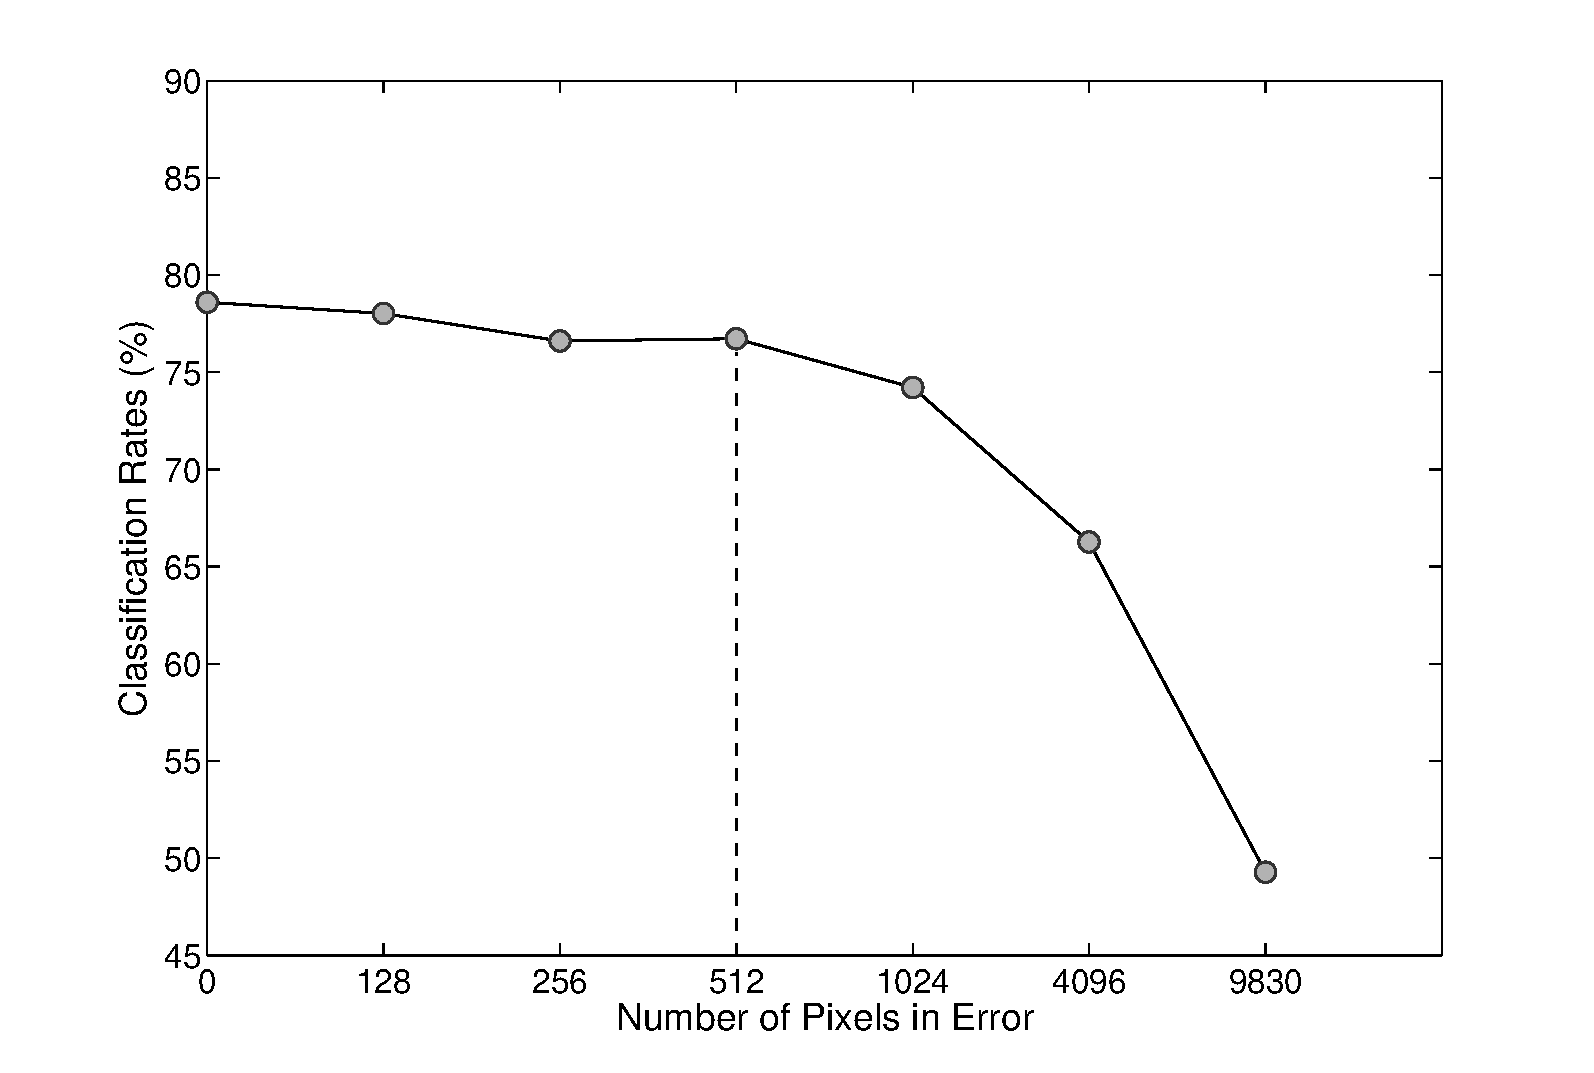
\includegraphics[width=1\linewidth,trim={20 20 30 20}, clip]{./figures/PixelSensitivityAnalysis.pdf}
\vspace{0pt}
\caption{HMAX resilience to errors. Six classes from CalTech101 were used. We observe a roll-off in accuracy beyond 512 pixels in error.}\label{fig:hmax_pixel_sensitivity}
\vspace{0pt}
\end{figure}

\subsection{Exploiting Resiliency for Compute Benefits}
In this section we explore the potential savings in computational work needed to be done while not compromising on accuracy. 
In embedded systems, compute resources come at a cost. Saving a few resources can enable 
fitting a design in a particular form-factor or may cause the design to overflow into the next larger generation of devices. 

Image reconstruction is an important processing technique in image processing and computer vision applications. Most object recognition algorithms use a multi-scale 
pyramid to make it scale invariant. For example, HMAX uses an image pyramid having 11 scales (including base scale of size $256\times256$) with a 
scale factor of $2^{1/4}$ and uses a bicubic interpolation technique 
to generate the image pyramid. The input image is first converted to grayscale and then passed through this image pyramid before computing the ``S1'' layer of HMAX. 

%Interpolation
\begin{figure*}[!htb]
\centering
\begin{tabular}{@{}c@{} @{}c@{}}
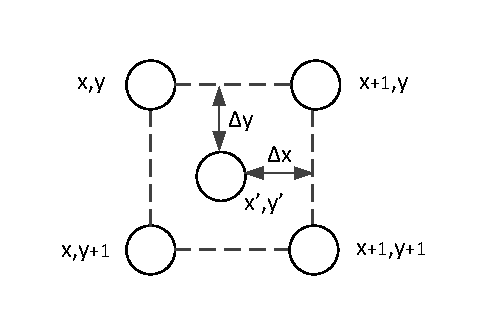
\includegraphics[width=0.3\textwidth]{./figures/bilinear.pdf} & 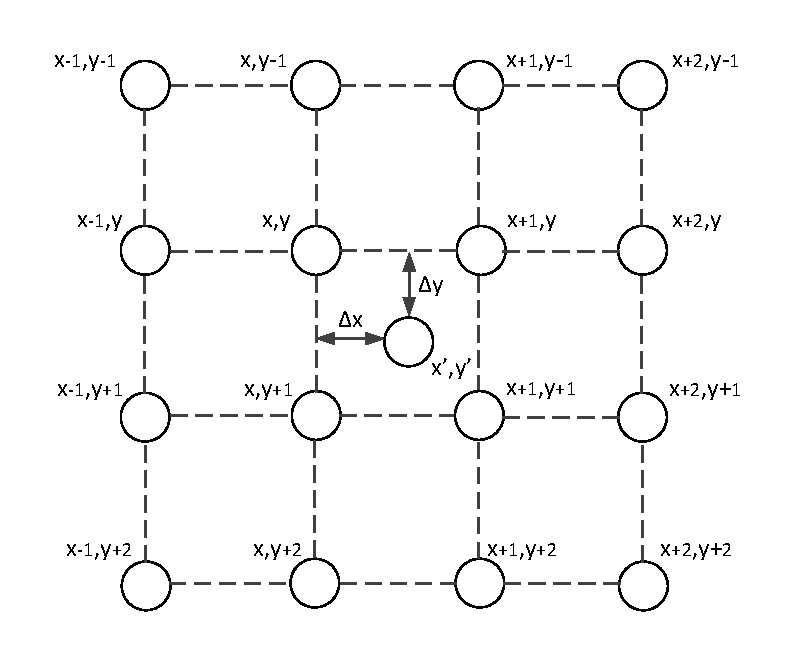
\includegraphics[width=0.5\textwidth]{./figures/bicubic.pdf}\\[\abovecaptionskip]
\small (a) Bilinear Interpolation & \small (b) Bicubic Interpolation
\end{tabular}
\vspace{1pt}
\caption{Interpolation techniques. In (a), four while in (b), 16 neighboring pixels are used for interpolating the value of the pixel at (x',y').}
\label{tab:interpolation}
\end{figure*}

Many architectures have been proposed to support linear 
and non-linear interpolation techniques~\cite{kesturdac}.
Given a pixel at $(x,y)$ with intensity $I(x,y)$, an interpolated pixel at $(x',y')$ at an offset of $(\Delta x, \Delta y)$ from $(x,y)$
(where $0<\Delta x,\Delta y<1$) can be computed using bilinear interpolation.
By definition, this involves computing two linear interpolations in the $x$ direction and one linear interpolation in the $y$ direction~\cite{IPHandbook}. 
This process, derived from first principles, is shown in ~(\ref{eq:1}) and requires eight multiplications. 
Fig.~\ref{tab:interpolation}(a) illustrates an interpolated pixel using four neighboring pixels.

\begin{equation}
\begin{split}
I(x',y') = &I(x,y) \times (1-\Delta x) \times (1-\Delta y) +\\ 
            &I(x+1,y) \times\Delta x \times (1-\Delta y) +\\ 
            &I(x,y+1) \times (1-\Delta x) \times\Delta y +\\ 
            &I(x+1,y+1) \times\Delta x \times\Delta y 
\end{split}
\label{eq:1}
\end{equation}

Using bicubic interpolation, the same interpolated pixel $I(x',y')$ is given by ~(\ref{eq:2}) where 
$R_c$ denotes a bicubic interpolation function~\cite{Keys}. The computation requires 56\footnote{Further optimizations are possible using shift and add operators but this would still require signficantly more multipliers than the bilinear version.} multiplications in all and Fig.~\ref{tab:interpolation}(b) shows the interpolated pixel 
using 16 neighboring pixels.

{\setstretch{0.25}
\begin{equation}
%\begin{split}
I(x',y')=\sum_{m=-1}^{2}\sum_{n=-1}^{2}I(x+m,y+n)R_c(m-\Delta x)R_c(-(n-\Delta y))
%\end{split}
\label{eq:2}
\end{equation}
}

We explored the capability of HMAX to correctly recognize objects using bilinear interpolation in the image pyramid. We used all 101 classes of CalTech101 
for this purpose. It should be noted that using the original bicubic interpolation technique, we achieve 54\% accuracy on the said dataset. This is in confirmation with the results shown in ~\cite{Mutch2008}. 
We then ran the experiment using bilinear interpolation and found the impact of this is a 1\% loss in accuracy. Thus, if the image pyramid is implemented 
using bilinear interpolation, we would need eight multipliers instead of 
56 multipliers. We tabulate our results in Table~\ref{table:compute}. These savings have a significant impact on area and performance of the accelerated system. 

\begin{table}[h]
\renewcommand{\arraystretch}{1.3}
\caption {Impact of Interpolation Techniques}
\label{table:compute}
\centering
\begin{tabular}{lllll}
 System & Algorithm & Accuracy & Multipliers\\\hline
 HMAX	& Bicubic   & 54\% & 56\\\hline
 HMAX   & Bilinear  & 53\% & 8\\\hline
\end{tabular}
\end{table}
